\section{valcheck.h File Reference}
\label{valcheck_8h}\index{valcheck.h@{valcheck.h}}


This graph shows which files directly or indirectly include this file:\nopagebreak
\begin{figure}[H]
\begin{center}
\leavevmode
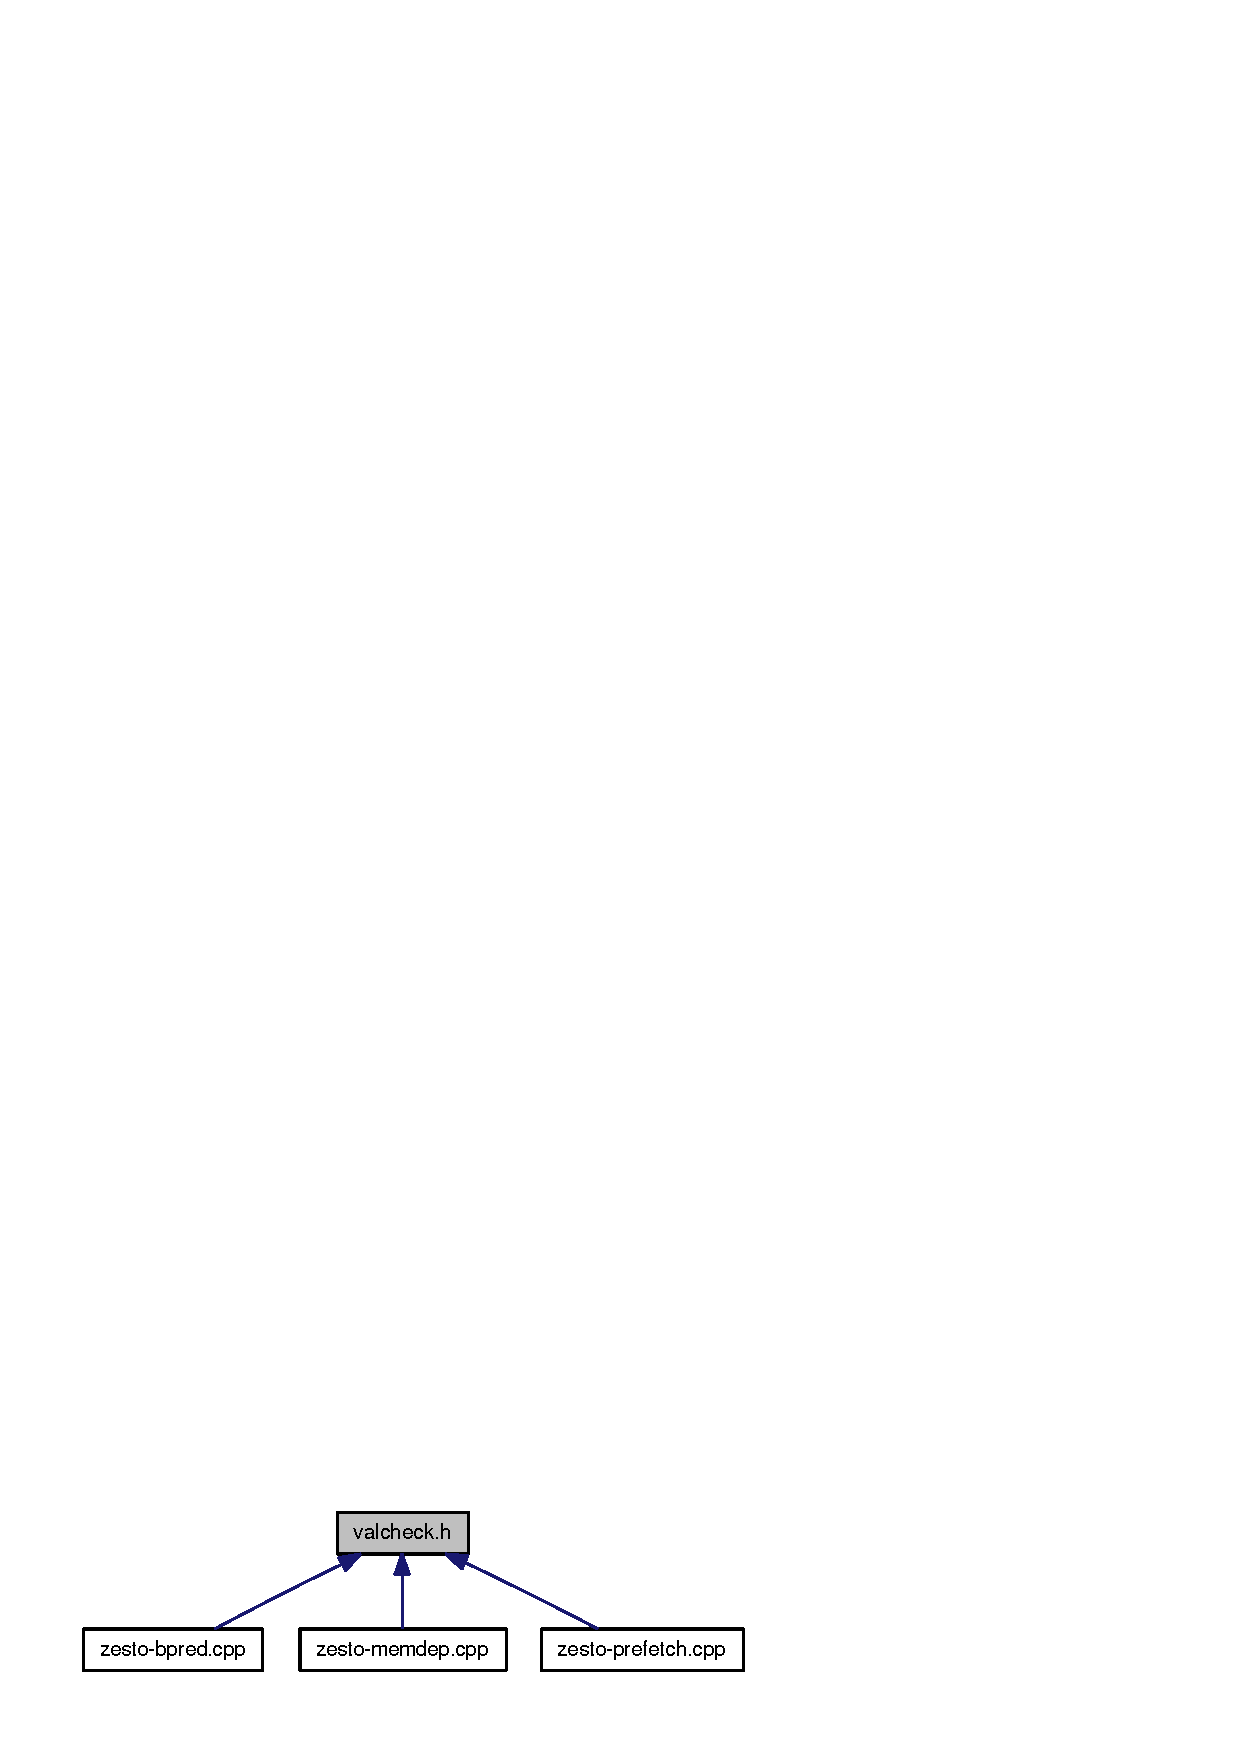
\includegraphics[width=180pt]{valcheck_8h__dep__incl}
\end{center}
\end{figure}
\subsection*{Defines}
\begin{CompactItemize}
\item 
\#define {\bf IS\_\-POW2}(x)~(!(((x)-1)\&(x)))
\item 
\#define {\bf CHECK\_\-POW2}(x)~if(!IS\_\-POW2(x)) fatal(\char`\"{}\%s(\%{\bf s}) \%{\bf s} must be a power of two.\char`\"{},name,COMPONENT\_\-NAME,\#x)
\item 
\#define {\bf CHECK\_\-PPOW2}(x)~if(!IS\_\-POW2(x) $|$$|$ ((x) $<$ 1)) fatal(\char`\"{}\%s(\%{\bf s}) \%{\bf s} must be a positive power of two.\char`\"{},name,COMPONENT\_\-NAME,\#x)
\item 
\#define {\bf CHECK\_\-NNEG}(x)~if(((x) $<$ 0)) fatal(\char`\"{}\%s(\%{\bf s}) \%{\bf s} must be non-negative.\char`\"{},name,COMPONENT\_\-NAME,\#x)
\item 
\#define {\bf CHECK\_\-POS}(x)~if(((x) $<$= 0)) fatal(\char`\"{}\%s(\%{\bf s}) \%{\bf s} must be positive.\char`\"{},name,COMPONENT\_\-NAME,\#x)
\item 
\#define {\bf CHECK\_\-NNEG\_\-LEQ}(x, y)~if(((x) $<$ 0) $|$$|$ ((x)$>$(y))) fatal(\char`\"{}\%s(\%{\bf s}) \%{\bf s} must be non-negative and less than or equal to \%lf.\char`\"{},name,COMPONENT\_\-NAME,\#x,(double)(y))
\item 
\#define {\bf CHECK\_\-POS\_\-LEQ}(x, y)~if(((x) $<$= 0) $|$$|$ ((x)$>$(y))) fatal(\char`\"{}\%s(\%{\bf s}) \%{\bf s} must be positive and less than or equal to \%lf.\char`\"{},name,COMPONENT\_\-NAME,\#x,(double)(y))
\item 
\#define {\bf CHECK\_\-NNEG\_\-LT}(x, y)~if(((x) $<$ 0) $|$$|$ ((x)$>$=(y))) fatal(\char`\"{}\%s(\%{\bf s}) \%{\bf s} must be non-negative and less than or equal to \%lf.\char`\"{},name,COMPONENT\_\-NAME,\#x,(double)(y))
\item 
\#define {\bf CHECK\_\-POS\_\-LT}(x, y)~if(((x) $<$= 0) $|$$|$ ((x)$>$=(y))) fatal(\char`\"{}\%s(\%{\bf s}) \%{\bf s} must be positive and less than or equal to \%lf.\char`\"{},name,COMPONENT\_\-NAME,\#x,(double)(y))
\item 
\#define {\bf CHECK\_\-POS\_\-GT}(x, y)~if(((x) $<$= 0) $|$$|$ ((x)$<$=(y))) fatal(\char`\"{}\%s(\%{\bf s}) \%{\bf s} must be positive and greater than \%lf.\char`\"{},name,COMPONENT\_\-NAME,\#x,(double)(y))
\item 
\#define {\bf CHECK\_\-BOOL}(x)~if(((x) != 0) \&\& ((x) != 1)) fatal(\char`\"{}\%s(\%{\bf s}) \%{\bf s} must be boolean (0 or 1).\char`\"{},name,COMPONENT\_\-NAME,\#x)
\end{CompactItemize}


\subsection{Define Documentation}
\index{valcheck.h@{valcheck.h}!CHECK\_\-BOOL@{CHECK\_\-BOOL}}
\index{CHECK\_\-BOOL@{CHECK\_\-BOOL}!valcheck.h@{valcheck.h}}
\subsubsection[{CHECK\_\-BOOL}]{\setlength{\rightskip}{0pt plus 5cm}\#define CHECK\_\-BOOL(x)~if(((x) != 0) \&\& ((x) != 1)) fatal(\char`\"{}\%s(\%{\bf s}) \%{\bf s} must be boolean (0 or 1).\char`\"{},name,COMPONENT\_\-NAME,\#x)}\label{valcheck_8h_e4da23c2826590bf3f9a30631991112a}




Definition at line 28 of file valcheck.h.

Referenced by bpred\_\-2lev\_\-t::bpred\_\-2lev\_\-t(), bpred\_\-bimode\_\-t::bpred\_\-bimode\_\-t(), bpred\_\-skewed\_\-t::bpred\_\-skewed\_\-t(), bpred\_\-yags\_\-t::bpred\_\-yags\_\-t(), and BTB\_\-2levbtac\_\-t::BTB\_\-2levbtac\_\-t().\index{valcheck.h@{valcheck.h}!CHECK\_\-NNEG@{CHECK\_\-NNEG}}
\index{CHECK\_\-NNEG@{CHECK\_\-NNEG}!valcheck.h@{valcheck.h}}
\subsubsection[{CHECK\_\-NNEG}]{\setlength{\rightskip}{0pt plus 5cm}\#define CHECK\_\-NNEG(x)~if(((x) $<$ 0)) fatal(\char`\"{}\%s(\%{\bf s}) \%{\bf s} must be non-negative.\char`\"{},name,COMPONENT\_\-NAME,\#x)}\label{valcheck_8h_add41af8cea1e110db7000fd5b0fb871}




Definition at line 14 of file valcheck.h.

Referenced by bpred\_\-2lev\_\-t::bpred\_\-2lev\_\-t(), bpred\_\-alloyedperceptron\_\-t::bpred\_\-alloyedperceptron\_\-t(), bpred\_\-bimode\_\-t::bpred\_\-bimode\_\-t(), bpred\_\-pathneural\_\-t::bpred\_\-pathneural\_\-t(), bpred\_\-perceptron\_\-t::bpred\_\-perceptron\_\-t(), bpred\_\-pwl\_\-t::bpred\_\-pwl\_\-t(), bpred\_\-skewed\_\-t::bpred\_\-skewed\_\-t(), bpred\_\-yags\_\-t::bpred\_\-yags\_\-t(), and fusion\_\-colt\_\-t::fusion\_\-colt\_\-t().\index{valcheck.h@{valcheck.h}!CHECK\_\-NNEG\_\-LEQ@{CHECK\_\-NNEG\_\-LEQ}}
\index{CHECK\_\-NNEG\_\-LEQ@{CHECK\_\-NNEG\_\-LEQ}!valcheck.h@{valcheck.h}}
\subsubsection[{CHECK\_\-NNEG\_\-LEQ}]{\setlength{\rightskip}{0pt plus 5cm}\#define CHECK\_\-NNEG\_\-LEQ(x, \/  y)~if(((x) $<$ 0) $|$$|$ ((x)$>$(y))) fatal(\char`\"{}\%s(\%{\bf s}) \%{\bf s} must be non-negative and less than or equal to \%lf.\char`\"{},name,COMPONENT\_\-NAME,\#x,(double)(y))}\label{valcheck_8h_dd6e150b6027f40ba3794f4ce8436f0e}




Definition at line 18 of file valcheck.h.\index{valcheck.h@{valcheck.h}!CHECK\_\-NNEG\_\-LT@{CHECK\_\-NNEG\_\-LT}}
\index{CHECK\_\-NNEG\_\-LT@{CHECK\_\-NNEG\_\-LT}!valcheck.h@{valcheck.h}}
\subsubsection[{CHECK\_\-NNEG\_\-LT}]{\setlength{\rightskip}{0pt plus 5cm}\#define CHECK\_\-NNEG\_\-LT(x, \/  y)~if(((x) $<$ 0) $|$$|$ ((x)$>$=(y))) fatal(\char`\"{}\%s(\%{\bf s}) \%{\bf s} must be non-negative and less than or equal to \%lf.\char`\"{},name,COMPONENT\_\-NAME,\#x,(double)(y))}\label{valcheck_8h_482b189474b5ba9954def6933e2fa0d1}




Definition at line 22 of file valcheck.h.\index{valcheck.h@{valcheck.h}!CHECK\_\-POS@{CHECK\_\-POS}}
\index{CHECK\_\-POS@{CHECK\_\-POS}!valcheck.h@{valcheck.h}}
\subsubsection[{CHECK\_\-POS}]{\setlength{\rightskip}{0pt plus 5cm}\#define CHECK\_\-POS(x)~if(((x) $<$= 0)) fatal(\char`\"{}\%s(\%{\bf s}) \%{\bf s} must be positive.\char`\"{},name,COMPONENT\_\-NAME,\#x)}\label{valcheck_8h_6302c4f5461fb1f977654eb1061ba9c8}




Definition at line 16 of file valcheck.h.

Referenced by bpred\_\-blg\_\-t::bpred\_\-blg\_\-t(), bpred\_\-tage\_\-t::bpred\_\-tage\_\-t(), BTB\_\-2levbtac\_\-t::BTB\_\-2levbtac\_\-t(), BTB\_\-btac\_\-t::BTB\_\-btac\_\-t(), and memdep\_\-lwt\_\-t::memdep\_\-lwt\_\-t().\index{valcheck.h@{valcheck.h}!CHECK\_\-POS\_\-GT@{CHECK\_\-POS\_\-GT}}
\index{CHECK\_\-POS\_\-GT@{CHECK\_\-POS\_\-GT}!valcheck.h@{valcheck.h}}
\subsubsection[{CHECK\_\-POS\_\-GT}]{\setlength{\rightskip}{0pt plus 5cm}\#define CHECK\_\-POS\_\-GT(x, \/  y)~if(((x) $<$= 0) $|$$|$ ((x)$<$=(y))) fatal(\char`\"{}\%s(\%{\bf s}) \%{\bf s} must be positive and greater than \%lf.\char`\"{},name,COMPONENT\_\-NAME,\#x,(double)(y))}\label{valcheck_8h_41b23373cb05c07ebb8aadb8dc2184e0}




Definition at line 26 of file valcheck.h.

Referenced by bpred\_\-tage\_\-t::bpred\_\-tage\_\-t().\index{valcheck.h@{valcheck.h}!CHECK\_\-POS\_\-LEQ@{CHECK\_\-POS\_\-LEQ}}
\index{CHECK\_\-POS\_\-LEQ@{CHECK\_\-POS\_\-LEQ}!valcheck.h@{valcheck.h}}
\subsubsection[{CHECK\_\-POS\_\-LEQ}]{\setlength{\rightskip}{0pt plus 5cm}\#define CHECK\_\-POS\_\-LEQ(x, \/  y)~if(((x) $<$= 0) $|$$|$ ((x)$>$(y))) fatal(\char`\"{}\%s(\%{\bf s}) \%{\bf s} must be positive and less than or equal to \%lf.\char`\"{},name,COMPONENT\_\-NAME,\#x,(double)(y))}\label{valcheck_8h_5d0c5afbebddacc12b87872ae081da05}




Definition at line 20 of file valcheck.h.

Referenced by bpred\_\-tage\_\-t::bpred\_\-tage\_\-t(), and fusion\_\-colt\_\-t::fusion\_\-colt\_\-t().\index{valcheck.h@{valcheck.h}!CHECK\_\-POS\_\-LT@{CHECK\_\-POS\_\-LT}}
\index{CHECK\_\-POS\_\-LT@{CHECK\_\-POS\_\-LT}!valcheck.h@{valcheck.h}}
\subsubsection[{CHECK\_\-POS\_\-LT}]{\setlength{\rightskip}{0pt plus 5cm}\#define CHECK\_\-POS\_\-LT(x, \/  y)~if(((x) $<$= 0) $|$$|$ ((x)$>$=(y))) fatal(\char`\"{}\%s(\%{\bf s}) \%{\bf s} must be positive and less than or equal to \%lf.\char`\"{},name,COMPONENT\_\-NAME,\#x,(double)(y))}\label{valcheck_8h_9aa4fef6ba728b734441f75c59066dac}




Definition at line 24 of file valcheck.h.

Referenced by bpred\_\-tage\_\-t::bpred\_\-tage\_\-t().\index{valcheck.h@{valcheck.h}!CHECK\_\-POW2@{CHECK\_\-POW2}}
\index{CHECK\_\-POW2@{CHECK\_\-POW2}!valcheck.h@{valcheck.h}}
\subsubsection[{CHECK\_\-POW2}]{\setlength{\rightskip}{0pt plus 5cm}\#define CHECK\_\-POW2(x)~if(!IS\_\-POW2(x)) fatal(\char`\"{}\%s(\%{\bf s}) \%{\bf s} must be a power of two.\char`\"{},name,COMPONENT\_\-NAME,\#x)}\label{valcheck_8h_de66ba7236859aa51477f42034673fc2}




Definition at line 10 of file valcheck.h.\index{valcheck.h@{valcheck.h}!CHECK\_\-PPOW2@{CHECK\_\-PPOW2}}
\index{CHECK\_\-PPOW2@{CHECK\_\-PPOW2}!valcheck.h@{valcheck.h}}
\subsubsection[{CHECK\_\-PPOW2}]{\setlength{\rightskip}{0pt plus 5cm}\#define CHECK\_\-PPOW2(x)~if(!IS\_\-POW2(x) $|$$|$ ((x) $<$ 1)) fatal(\char`\"{}\%s(\%{\bf s}) \%{\bf s} must be a positive power of two.\char`\"{},name,COMPONENT\_\-NAME,\#x)}\label{valcheck_8h_c99c690e4a721f3296ab6329a6dbaebf}




Definition at line 12 of file valcheck.h.

Referenced by bpred\_\-2bC\_\-t::bpred\_\-2bC\_\-t(), bpred\_\-2lev\_\-t::bpred\_\-2lev\_\-t(), bpred\_\-alloyedperceptron\_\-t::bpred\_\-alloyedperceptron\_\-t(), bpred\_\-bimode\_\-t::bpred\_\-bimode\_\-t(), bpred\_\-blg\_\-t::bpred\_\-blg\_\-t(), bpred\_\-pathneural\_\-t::bpred\_\-pathneural\_\-t(), bpred\_\-perceptron\_\-t::bpred\_\-perceptron\_\-t(), bpred\_\-pwl\_\-t::bpred\_\-pwl\_\-t(), bpred\_\-skewed\_\-t::bpred\_\-skewed\_\-t(), bpred\_\-tage\_\-t::bpred\_\-tage\_\-t(), bpred\_\-yags\_\-t::bpred\_\-yags\_\-t(), BTB\_\-2levbtac\_\-t::BTB\_\-2levbtac\_\-t(), BTB\_\-btac\_\-t::BTB\_\-btac\_\-t(), fusion\_\-colt\_\-t::fusion\_\-colt\_\-t(), fusion\_\-mcfarling\_\-t::fusion\_\-mcfarling\_\-t(), fusion\_\-multihybrid\_\-t::fusion\_\-multihybrid\_\-t(), fusion\_\-priority\_\-t::fusion\_\-priority\_\-t(), memdep\_\-lwt\_\-t::memdep\_\-lwt\_\-t(), prefetch\_\-context\_\-t::prefetch\_\-context\_\-t(), and prefetch\_\-IP\_\-t::prefetch\_\-IP\_\-t().\index{valcheck.h@{valcheck.h}!IS\_\-POW2@{IS\_\-POW2}}
\index{IS\_\-POW2@{IS\_\-POW2}!valcheck.h@{valcheck.h}}
\subsubsection[{IS\_\-POW2}]{\setlength{\rightskip}{0pt plus 5cm}\#define IS\_\-POW2(x)~(!(((x)-1)\&(x)))}\label{valcheck_8h_fd922d5a863aa3844c5390af42d97638}




Definition at line 7 of file valcheck.h.